% File: T.tex
% Created: 2014-11-07
% Author: Tesser Paolo
% Email: p.tesser921@gmail.com
%
%
% Modification History
% Version	Modifier Date	Author			Change
% ====================================================================
% 0.0.1		2014-11-07		Tesser-Paolo	inserita sezione
% ====================================================================
% 0.0.2		2015-03-18		Tesser Paolo	inserito vocabolo: Tecniche di analisi
% ====================================================================
%

\section{T} % (fold)
\label{sec:t}
	\begin{itemize}
		\item \textbf{Tecniche di analisi}: [IS] ci sono diversi approcci per analizzare i bisogni e le fonti di un progetto. Attraverso lo studio del dominio, andando quindi ad osservare i comportamenti dell'utente finale e dell'ambiente d'uso immergendosi nei panni degli utilizzatori. Interagendo con il cliente in maniera il meno invasiva possibile e facendolo in modo strutturato e rendicontabile. Un'altra tecnica è quella di avere dei brain-storming, ma per farlo bisogna che:
			\begin{itemize}
				\item ci sia un gruppo di persone che sono consapevoli di ciò che stanno facendo;
				\item serve un'altra persona che fa da controllore, fissa l'agenda, il tempo e la scaletta;
				\item serve una persona che tenga le minute, cioè i punti salienti.
			\end{itemize}
		\noindent
		Infine può essere fatta anche della prototipazione, che può essere interna (per capire meglio le cose) o esterna (per chiedere al cliente se ciò che sta domandando);

		\item \textbf{Teorema di Dijkstra (1969)}: [VV][analisi dinamica] il test di un programma può rilevare la presenza di malfunzionamenti, ma non dimostrarne l'assenza;

		\item \textbf{Teorema di Howden (1975)}: [VV][analisi dinamica] non esiste un algoritmo che, dato un programma P qualsiasi, generi per esso un test finito ideale;

		\item \textbf{Test}: [VV][analisi dinamica]
			\begin{figure}[htbp]
				\centering
				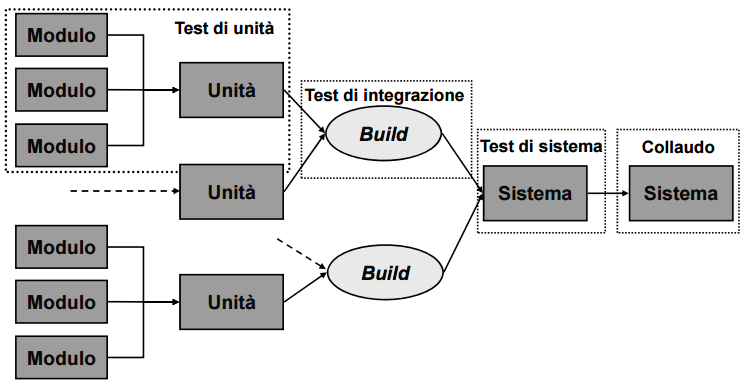
\includegraphics[scale=0.5]{img/composizione_test.png}
				\caption{Composizione Test}
				\label{fig:comp_test}
			\end{figure}

			\begin{itemize}
				\item \textbf{test di unità}: attività di analisi dinamica che si può svolgere con il massimo grado di parallelismo in quanto coinvolge la più piccola parte non ulteriormente scomponibile di un programma. La responsabilità è dello stesso programmatore per le unità più semplici, altrimenti di un verificatore autonomo. Nel primo caso infatti potrebbe esserci conflitto di interesse, meglio quindi peer-programming. Sono i test più costosi. Unità e moduli vengono determinati durante la progettazione di dettaglio e conseguentemente anche il piano di test. La TU è completa quando ha verificato tutte le unità. Piuttosto di tagliare i test di unità, è meglio che il Responsabile di Progetto, tagli i requisiti opzionali. Possono essere di due tipi:
					\begin{itemize}
						\item \textbf{test funzionale (black-box)}: guarda solo l'uscita. Da solo non può accertare correttezza e completezza della logica interna dell'unità. Va quindi necessariamente integrato con test strutturali. Fa riferimento alla specifica dell'unità e utilizza dati di ingresso capaci di provocare l'esito atteso. Si usano delle le classi di equivalenza per non avere infiniti valori di ingresso;
						\item \textbf{test strutturale (white-box)}: verifica la logica interna del codice dell'unità cercando massima copertura. Ciascuna prova deve essere progettata per attivare ogni cammino di esecuzione all'interno del modulo. Ciascuno insieme di dati di ingresso che attivano un percorso costituiscono un caso di prova.
					\end{itemize}

				\item \textbf{test di integrazione}: servono per verificare la costruzione incrementale del sistema. Può essere in parallelo per i componenti che non collaborano tra di loro. In condizioni ottimali, l'integrazione dovrebbe essere prova di problemi. Viene applicata alla componenti specificate nella progettazione architetturale. La loro integrazione costituisce il sistema completo. I problemi che si rilevano durante questi test manifestano difetti di progettazione o insufficiente qualità nei test di unità. Si inizia a integrare la componente che ha meno dipendenze.

				\item \textbf{test di sistema e collaudo}: i primi sono svolti internamente dal fornitore per accertare la copertura dei requisiti SW, mentre i secondi sono supervisionati dal committente per dimostrare la conformità del prodotto sulla base di casi di prova specificati nel o implicati dal contratto. I primi sono di tipo funzionale (black-box) in quanto non dovrebbero richiedere conoscenza della logica interna del software.

				\item \textbf{test di regressione}: rappresentano l'insieme di test necessari ad accertare che la modifica di una parte P di S non causi errori in P o nelle altre parti di S che dipendono da P. Il rischio che degli errori si verifichino cresce tanto più cresce l'accoppiamento fra le diverse parti e al diminuire dell'accoppiamento.

			\end{itemize}







		\item \textbf{Tracciamento dei requisiti}: [DOC] ha il compito di fissare le relazioni tra i prodotti del processo di sviluppo. Vengono usate delle matrici di tracciabilità. Il tracciamento viene fatto in avanti (forward) che indica la completezza e all'indietro (backward) che indica la necessità. I tracciamenti necessari sono i seguenti:
			\begin{itemize}
				\item requisiti utente (capitolato) <-> requisiti software (AdR)
				\item requisiti software <-> descrizione dei componenti (ST)
				\item test di unità <-> moduli di disegno di dettaglio (DdP)
				\item test di integrazione <-> componenti architetturali
				\item test di sistema <-> requisiti software
				\item test di accettazione <-> requisiti utente
			\end{itemize}

	\end{itemize}
% section t (end)